%! Author = ryanb
%! Date = 10/31/2025

% Preamble
\documentclass{amsart}

% Packages
\usepackage{amsmath}
\usepackage{amsrefs}
\usepackage{amsthm}

\usepackage{lipsum}
\usepackage{tikz} % delete when finished
\usepackage{float}

\usetikzlibrary{backgrounds}

\theoremstyle{definition}
\newtheorem{definition}{Definition}[section]

\theoremstyle{plain}
\newtheorem{theorem}{Theorem}[section]


% Document
\begin{document}

    \title{Our Title}
    \author{Ryan Bruno}
    \author{Lucas Johnson}
    \author{Nathan LaCrosse}
    \author{Nick Proctor}
    \date{\today}

    \begin{abstract}
        \lipsum[1]
    \end{abstract}

    \maketitle

    \tableofcontents % uncomment if needed

    \section{Introduction to Planar Graphs}\label{sec:intro}

    \begin{definition}
        A graph $G$ is called a \emph{planar graph} if $G$ can be drawn in the plane without any two of its edges crossing~\cite{ourBook}.
        If $G$ is already drawn in the plane without crossings, then $G$ is a \emph{plane graph}.
    \end{definition}
    Importantly, any graph isometric to a plane graph is therefore planar.
    \begin{center}
        \begin{figure}[H]
            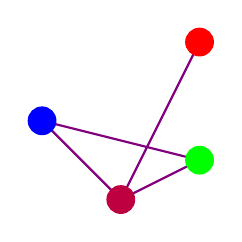
\begin{tikzpicture}[scale=0.5]
                \draw[violet, thick] (0,2) -- (2,0);
                \draw[violet, thick] (2,0) -- (4,1);
                \draw[violet, thick] (4,1) -- (0,2);
                \draw[violet, thick] (2,0) -- (4,4);

                \filldraw [blue] (0, 2) circle (10pt);
                \filldraw [purple] (2, 0) circle (10pt);
                \filldraw [green] (4, 1) circle (10pt);
                \filldraw [red] (4, 4) circle (10pt);
            \end{tikzpicture}
            \hspace{1in}
            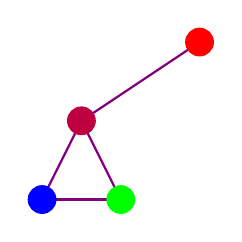
\begin{tikzpicture}[scale=0.5]
                \draw[violet, thick] (0,0) -- (2,0);
                \draw[violet, thick] (2,0) -- (1,2);
                \draw[violet, thick] (1,2) -- (0,0);
                \draw[violet, thick] (1,2) -- (4,4);

                \filldraw [blue] (0, 0) circle (10pt);
                \filldraw [purple] (1, 2) circle (10pt);
                \filldraw [green] (2, 0) circle (10pt);
                \filldraw [red] (4, 4) circle (10pt);
            \end{tikzpicture}\caption{The planar graph on the left is planar since it is isomorphic to the plane graph on the right.}\label{fig:isomorphicPlanar}
        \end{figure}
    \end{center}
    From here on, when referring to planar graphs, we will be considering the plane graph that the graph is isomorphic to.
    Often, when working with planar graphs, one is concerned with whether or not a given graph is planar.
    This question appears often in contexts where there are connections on a $2D$ gid and intersections are impossible.

    In order to solve this, we must discuss what properties define a planar graph.
    One important theorem is the Euler Identity.

    \begin{theorem}[The Euler Identity~\cite{ourBook}]
        For every connected plane graph of order $n$, size $m$ and having $r$ regions,
        \[n-m+r=2.\]
    \end{theorem}

    In order to be able to understand this theorem, let us first discuss the regions of a graph.
    A \emph{region} is an area bounded by the edges and vertices of a graph $G$.
    Additionally, there is an external region which is unbounded.
    \begin{figure}[H]
        \centering
        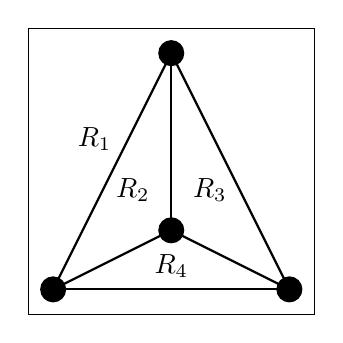
\begin{tikzpicture}[scale=0.75, show background rectangle]
            \draw[black, thick] (0,0) -- (2,4);
            \draw[black, thick] (0,0) -- (2,1);
            \draw[black, thick] (0,0) -- (4,0);

            \draw[black, thick] (2,1) -- (2,4);
            \draw[black, thick] (2,1) -- (4,0);

            \draw[black, thick] (2,4) -- (4,0);

            \filldraw [black] (2, 1) circle (6pt);
            \filldraw [black] (4, 0) circle (6pt);
            \filldraw [black] (0, 0) circle (6pt);
            \filldraw [black] (2, 4) circle (6pt);

            \node[above=0.75in, right=0.075in] at (0,0) {$R_1$};
            \node[above=0.2in, left=0.06in] at (2,1) {$R_2$};
            \node[above=0.2in, right=0.06in] at (2,1) {$R_3$};
            \node at (2,0.4) {$R_4$};
        \end{tikzpicture}
        \caption{A planar graph with its regions denoted.}
        \label{fig:regions}
    \end{figure}

    With this in mind, let us prove Euler's Identity.
    \begin{proof} Proceed by induction.
        \begin{enumerate}
            \item \emph{Base Case:} Consider the graph $K_1$, of order $1$, size $0$ and containing one region.
                Since there are no possible edges that could cross, the induction holds.
            \item \emph{Inductive Hypothesis:} If we assume that the hypothesis holds for a graph of order $n$, size $m$ and $r$ regions, then we will show it holds for a graph of order $n$, size $m=1$ and
        \end{enumerate}
    \end{proof}

    ??

    \newpage

    % bibliography stuff goes here
    \begin{bibdiv} % "produces the chapter or section heading for the bibliography" (the thing that says 'REFERENCES')
        \begin{biblist} % contains the reference list

            % may add more data to this
            \bib{ourBook}{book}{
                title={Graphs and Digraphs},
                author={Gary Chartrand},
                author={Linda Lesniak},
                author={Ping Zhang},
                date={2016},
                publisher={CRC Press},
                address={Boca Raton}
            }

        \end{biblist}
    \end{bibdiv}

\end{document}
